
\begin{figure}[h!]
  \centering
  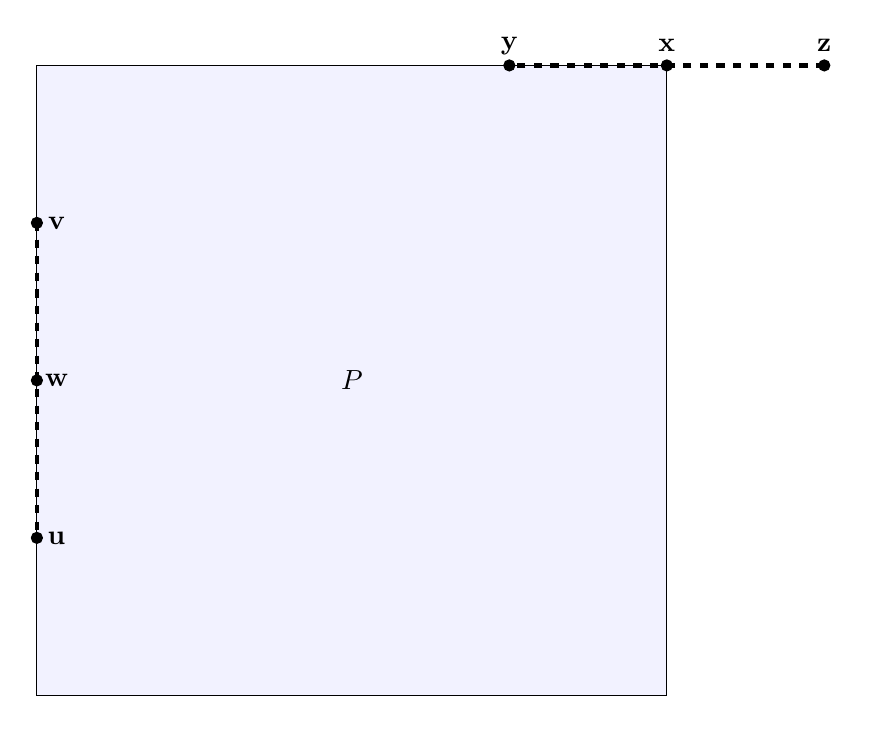
\begin{tikzpicture}
    \tikzset{punkt/.style={point, draw=black}}
    
    
%Punkter

	\node at (4,4)	(1){};
	\node at (-4,4)	(4){};
	\node at (4,-4)	(2){};
	\node at (-4,-4) (3){};


	\filldraw[black, fill=blue!5] (2) rectangle (4);
	\node at (0,0) (P){$P$};
	
	\filldraw [black] (2,4) circle (2pt);
	\filldraw [black] (4,4) circle (2pt);
	\filldraw [black] (6,4) circle (2pt);
	\filldraw [black] (-4,2) circle (2pt);
	\filldraw [black] (-4,0) circle (2pt);
	\filldraw [black] (-4,-2) circle (2pt);	
	\node at (2,4.25)	 (y){$\textbf{y}$};
	\node at (4,4.25)	 (x){$\textbf{x}$};
	\node at (6,4.25)	 (z){$\textbf{z}$};
	\node at (-3.75,2)  (v){$\textbf{v}$};
	\node at (-3.75,0)	 (w){$\textbf{w}$};
	\node at (-3.75,-2) (u){$\textbf{u}$};


	\draw[-, dashed,black,ultra thick] (6,4) -- (2,4);
	\draw[-, dashed,black,ultra thick] (-4,2) -- (-4,-2);

  \end{tikzpicture}
  \caption{En afgrænset polytop $P$ hvor $\textbf{x}$ er et ekstramapunkt da der ikke findes vektorer $\textbf{y}$ og $\textbf{z}$ sådan at $\mathbf{x}=\lambda\mathbf{y}+(1-\lambda)z$. $\textbf{w}$ er i modsætning ikke et ekstremapunkt da der findes $\textbf{v}$ og $\textbf{u}$ sådan at $\mathbf{w}=\lambda\mathbf{v}+(1-\lambda)u$.}
  \label{fig:ekstrema}
\end{figure}
%
%
%    \node[punkt] at (-4,0.5)      (v1){$v_1$};
%    \node[punkt] at (-2,0.5)      (v2){$v_2$};
%    \node[punkt] at (-4,-1.5)     (v3){$v_3$};
%    \node[punkt] at (-2,-1.5)     (v4){$v_4$};
%    \node at (-3,2)     (v){$K_{4}$};
%
%
%    \node[punkt] at (4.6,-0.2)      (k1){$v_3$};
%    \node[punkt] at (1.4,-0.2)      (k2){$v_2$};
%    \node[punkt] at (2,-2)     (k3){$v_4$};
%    \node[punkt] at (4,-2)     (k4){$v_5$};
%    \node[punkt] at (3,1)      (k5){$v_1$};
%    \node at (3,2)      (k){$K_{5}$};
%
%
%
%
%
%    \draw [-, thick, draw=black] (v1) -- (v2);
%    \draw [-, thick, draw=black] (v1) -- (v3);
%    \draw [-, thick, draw=black] (v1) -- (v4);
%    \draw [-, thick, draw=black] (v2) -- (v3);
%    \draw [-, thick, draw=black] (v2) -- (v4);
%    \draw [-, thick, draw=black] (v3) -- (v4);